\documentclass{scrartcl}			% defines the kind of document you want to produce

% Include different packages:
\usepackage[utf8]{inputenc}
\usepackage[T1]{fontenc}
\usepackage{lmodern}
\usepackage[english]{babel}
\usepackage{amsmath}
\usepackage{float}
\usepackage{graphicx}           	% include graphics
\usepackage{caption}
\usepackage{subcaption}
\usepackage{hyperref}
\usepackage{listings}
\usepackage{fancyvrb}

\title{Neuroprothetik Exercise 5 \\\textsl{}
	Multicompartment Model}

\author{Aleksandra Teska}
\date{24. June 2018}


\begin{document} 					% Document begins here

\maketitle
\section{Multicompartment Model}

In this exercise the Hodgkin \& Huxley  neuron Model was adapted into multicompartment model consisting of 100 compartments. The backward Euler method was used to solve the system of differential equations. The exponential-euler solver was used to solve the gating ODEs.

\section{Experiments}		% start a new sectio
The implemented model was then used for simulations. Simulations were 100 ms long ( with ${\Delta t = 25 \mu s}$) at 6.3$^{\circ}$C with the following settings:

\begin{enumerate}
	\item Stimulate the axon at the first compartment with a rectangular 5 ms long pulse with an amplitude of 10$\mu A/cm^2$. Visualize how the action potential propagates along the axon.
	\item Stimulate the axon with the same pulse as above but at compartment 20 and simultaneously at compartment 80. 
	\item Explore the different parameters of the model and find out which would affects the speed of action potential propagation.
\end{enumerate}

\subsection{Analysis of the Results}
In the first simulation we could see the action potential propagating through the axon from the original 1st compartment. \\

When the compartments 20 and 80 were stimulated simultaneously the resulting propagating profile differed.
Both of those compartments were connected to two corresponding compartments and because of that the action their potential was propagated in two directions (two V-shapes on the Figure \ref{fig2}). When the two propagated potentials with different directions met around compartment 50 , due to opposite direction of propagation, they stopped the further propagation of both of them.\\

Additionally, different parameters of the model were explored in order to find out which of them would affects the speed of action potential propagation. Time constant tau for each compartment is defined as:
\begin{align}
\tau = \frac{1}{R * C}
\end{align}
Therefore changing both the capacity or any parameter that contributes to the resistance value ( $\rho_{axon}$, $r_{axon}$, $l_{comp}$ ).

\newpage
\section{Plots}
\begin{figure}[hbpt!]					%start figure-environment
	\begin{flushleft}
		\hspace*{-0.3in}
		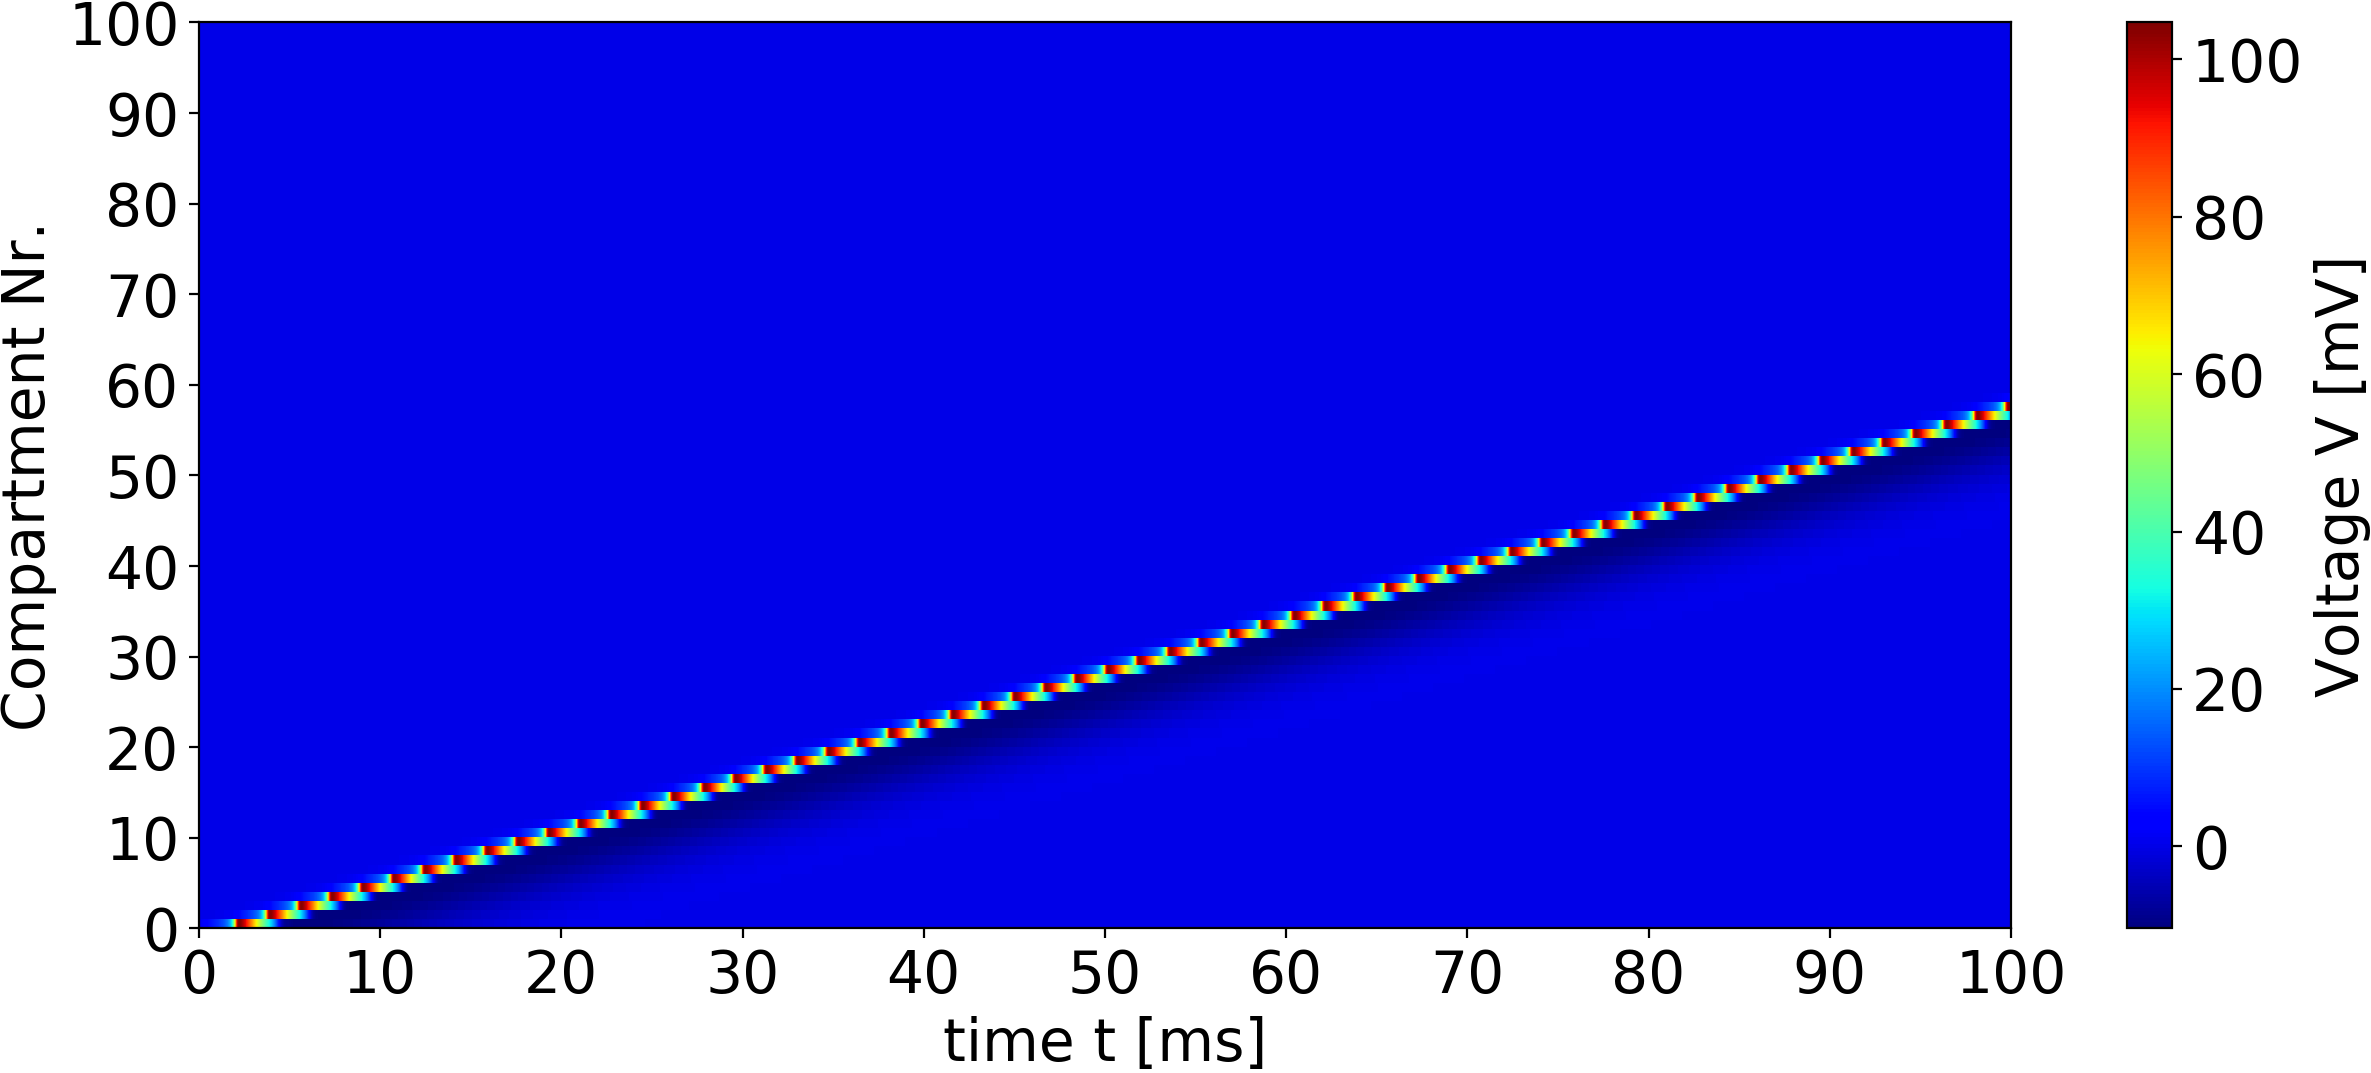
\includegraphics[scale=0.53]{1.png}
		\captionsetup{width=\linewidth}  %choose the with of the caption
		\caption{First experiment, stimulation of the first compartment with a rectangular 5ms long pulse with an amplitude of 10$\mu A/cm^2$, visualization of propagation through the axon.}		
		\label{fig1} %choose a label, see subsection references
	\end{flushleft}
\end{figure}

\begin{figure}[hbpt!]					%start figure-environment
	 \begin{flushleft}
		\hspace*{-0.3in}
		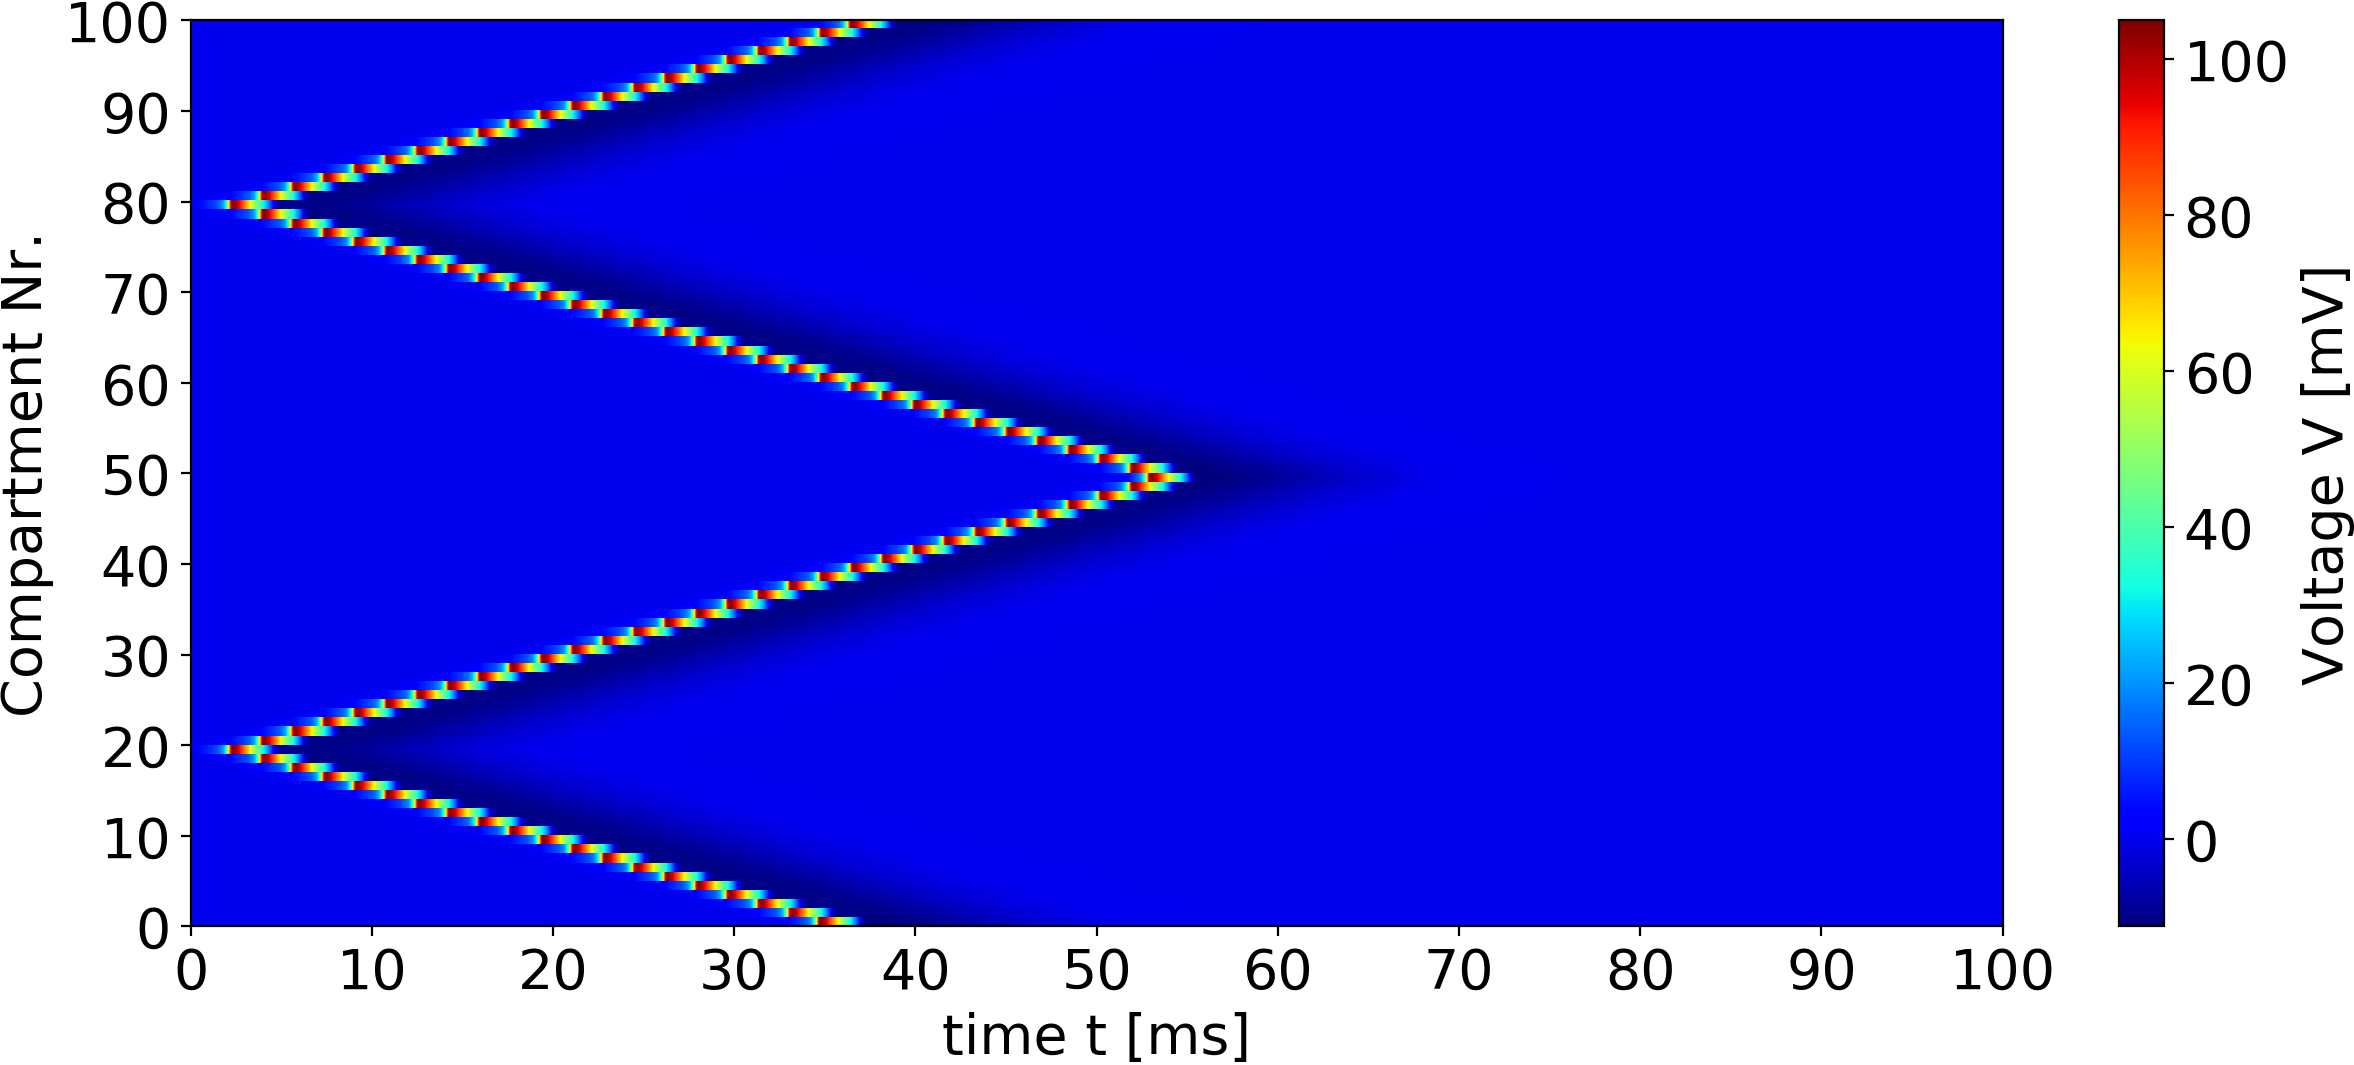
\includegraphics[scale=0.53]{2.png}
		\captionsetup{width=\linewidth}  %choose the with of the caption
		\caption{Second experiment, stimulation of the 20th and 80th compartments with a rectangular 5ms long pulse with an amplitude of 10$\mu A/cm^2$, visualization of propagation through the axon.}		
		\label{fig2} %choose a label, see subsection references
	\end{flushleft}
\end{figure}

\end{document}
